\chapter{Testing}
\label{chap:testing}

\section{Graph View Performance}

The graph can handle the entire CitHep dataset and, thanks to dynamic loading, could handle even larger graphs.
In Figure \ref{obr:afantazie_cithep_highlighted_thought}, one can see a highlighted thought from the \gls{cithep_dataset} dataset.

To achieve this, we wrote a C\# script to import the CitHep data files into the Aphantasia database.
In the graph view, we used the same parameter settings we used for the much smaller graphs in \gls{production} environment, which at the time consisted of around 600 and 150 thoughts, respectively.
To our surprise the resulting graph behaved well and except for increased tendency to jitter the CitHep graph view was smooth and stable.
The only parameter we had to change was neighborhood \gls{BFS} depth - from three down to just one.
CitHep graph is bigger and much more interconnected than the small production graphs, so even at depth two, the graph exploration feature often resulted in an unreasonable amount of on-screen nodes.

\subsection{Limits of the Graph View}

In Figure \ref{obr:afantazie_cithep_3k}, we have seen how Aphantasia handles 3 000 nodes
even before the dynamic loading was implemented. 

The application is not meant to display large graphs at once, but out of curiosity we tried to render as many thoughts as possible.

First, we tried to set the on-screen thought limit to 40 000
(and thus load and render the entire \gls{cithep_dataset} dataset) and we were not able to fetch the data from the backend.
We are not sure why this happened but one possible explanation is that the API response is too large and either the server and/or the client were not able to handle it.

In the second test we set the on-screen thought limit to 10 000 and we were able to fetch the data and render it.
The result was not unexpected - a big hairball of nodes and edges running at less than one frame per second.
See Figure \ref{obr:afantazie_cithep_10000_on-screen-limit}.


\begin{figure}[p]
    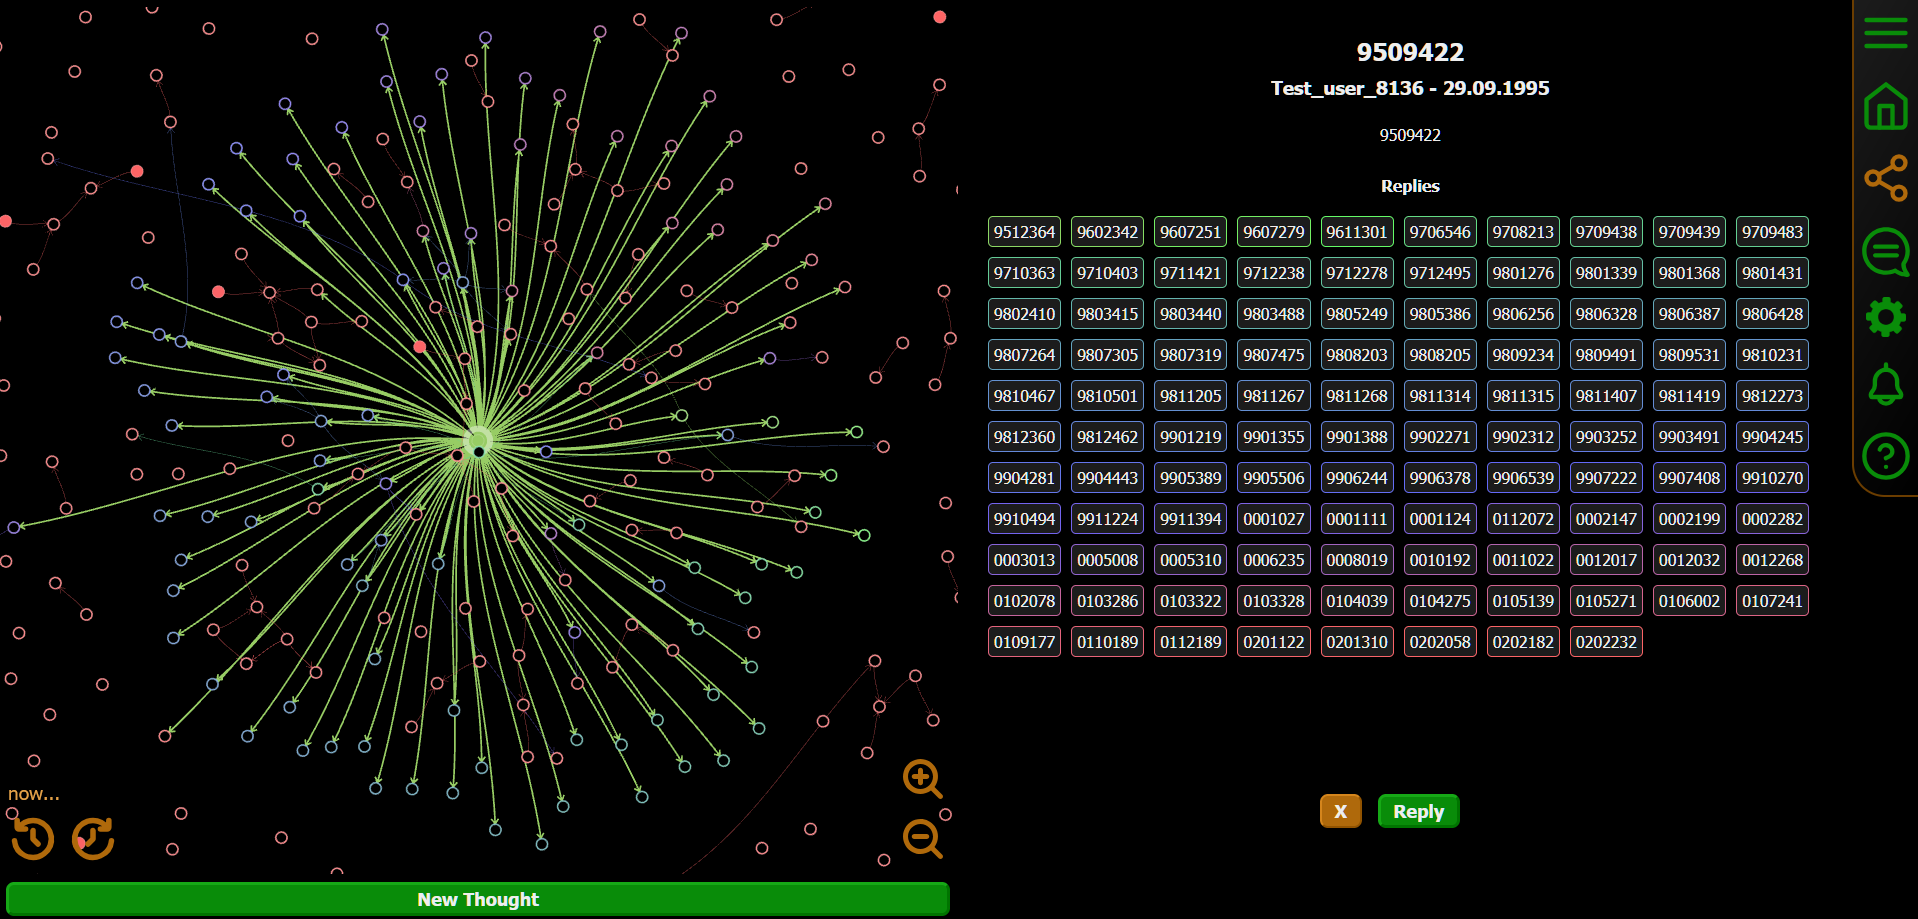
\includegraphics[width=130mm, keepaspectratio]{img/afantazie_cithep_highlighted_thought.png}
    \caption{A highlighted thought of the CitHep Dataset in Aphantasia}
    \label{obr:afantazie_cithep_highlighted_thought}
\end{figure}

\begin{figure}[p]
    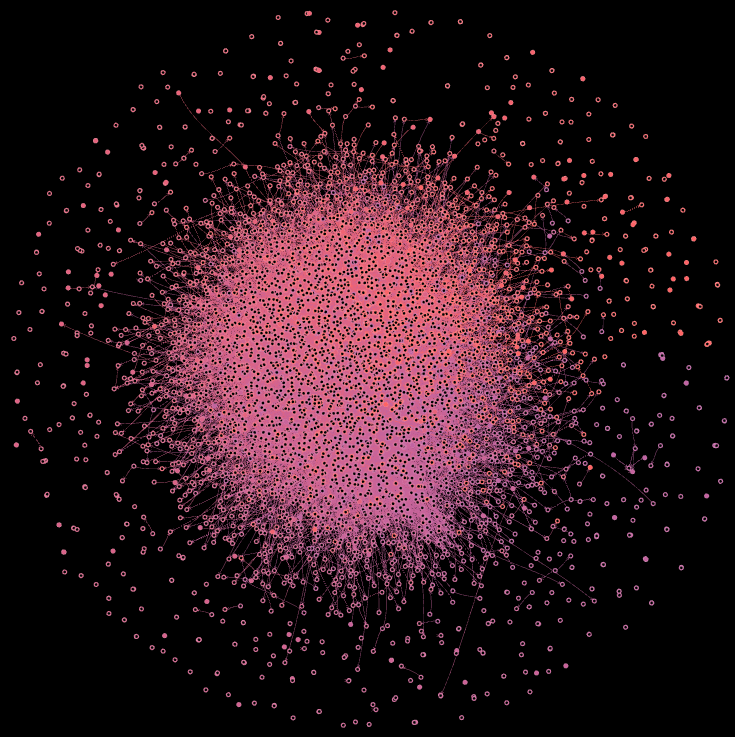
\includegraphics[width=130mm, keepaspectratio]{img/afantazie_cithep_10000_on-screen-limit.png}
    \caption{Cithep dataset rendered in Aphantasia with 10000 on-screen thought limit}
    \label{obr:afantazie_cithep_10000_on-screen-limit}
\end{figure}

From our tests, we learned that Aphantasia's performance begins to degrade noticeably at around 400-700 on-screen thought limit
and gradually drops to just a few frames per second with the limit set to around 1 500.
These values are highly dependent on the connectivity of the data, with more connections leading to more computation time and thus lower performance.

\section{User Feedback}
We advertised the application on Reddit, sharing both the Czech and English versions across several subreddits.

Most comments were positive, praising the application's concept and the experience of exploring thoughts
with one user describing the experience as feeling like an "archeologist" uncovering ideas.

Negative feedback focused on the lack of practicality, outdated UI, and occasional bugs.
Users also suggested missing features such as pinch zoom, image posting, a better landing page, and filtering.
Browser compatibility issues were mentioned as well.

The feedback was mostly constructive, and we are grateful for it.
It helped us hone on the experience users already found fun and stimulating, specifically interaction and exploration.
However, some users admitted they did not understand the application, highlighting the need for a proper tutorial.

\section{Aphantasia Versus Related Software}

Ideologically, Aphantasia is closest to Obsidian.
There is of course an obvious difference between the two - Obsidian is local note-taking system with graph view while Aphantasia is an online social experience based on graph view.
Both are, however, meant for the general audience, and their graph views bear a similarity.

Compared to Gephi and Cytoscape.js, Aphantasia has lower performance on large graphs rendered at once.
However, thanks to the time slider and graph exploration features, it can handle much larger datasets in an intuitive way.
The dynamic loading could, in theory, handle millions of nodes. In such case the main limiting factor would be the performance of the backend and the database.

Finally, in table \ref{tab:comparison_2}, we added Aphantasia to the comparison table from the first chapter.
We can see that Aphantasia is a good compromise between the ease of use of Obsidian
and the performance of Gephi and Cytoscape.js.

\begin{table}[ht]
    \centering
    \caption{Comparison of Obsidian, Gephi, Cytoscape.js and Aphantasia}
    \label{tab:comparison_2}
    \begin{tabularx}{\textwidth}{|l|X|X|X|X|}
        \hline
        \textbf{}                     & \textbf{Obsidian}       & \textbf{Gephi}                      & \textbf{Cytoscape}                & \textbf{Aphantasia} \\ \hline
        \textbf{Use-case}             & note-taking             & data analysis and visualization     & graph visualization in browser    & social network \\ \hline
        \textbf{Target}               & general                 & researchers,                        & web                               & general \\ 
        \textbf{Userbase}             &  audience               & technical users                     & developers                        & audience, graph enthusiasts \\ \hline
        \textbf{User}                 & easy to use             & technical,                          & program-                          & intuitive, \\
        \textbf{Experience}           &                         & steep learning curve                & matic, mostly parametrization     & slight learning curve\\ \hline
        \textbf{3 000 nodes}          & slow                    & stable,                             & stable but                        & stable, \\ 
        \textbf{handling}             & indexing but smooth afterwards & smooth                              & visibly lower FPS                 & smooth, explorable \\ \hline
        \textbf{34 546 nodes}         & skipped as              & mostly                              & crashed                           & stable, \\ 
        \textbf{handling}             & indexing took too long  & stable, lower FPS while running FDL & immediately                       & explorable, slightly increased jitter \\ \hline
    \end{tabularx}
\end{table}